\documentclass[tikz,border=10pt]{standalone}
\begin{document}
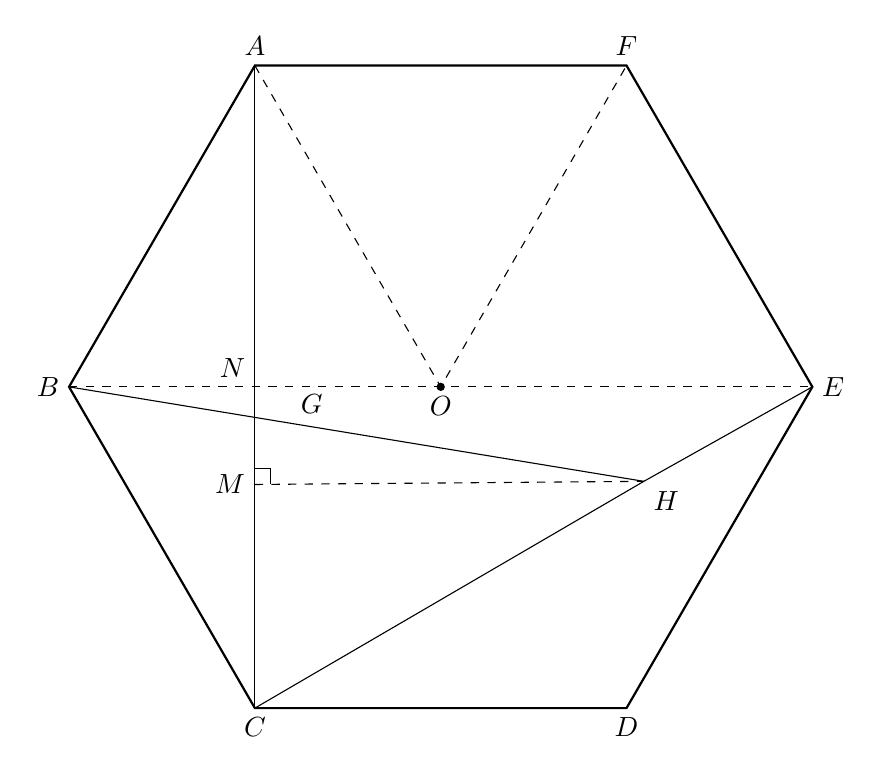
\begin{tikzpicture}[scale=1]
  \coordinate (A) at (-2.36,4.08);
  \coordinate (F) at (2.36,4.08);
  \coordinate (B) at (-4.72,0);
  \coordinate (E) at (4.72,0);
  \coordinate (C) at (-2.36,-4.08);
  \coordinate (D) at (2.36,-4.08);
  \coordinate (O) at (0,0);
  \coordinate (N) at (-2.36,0);
  \coordinate (M) at (-2.36,-1.24);
  \coordinate (H) at (2.58,-1.20);
  \coordinate (G) at (-1.9,-0.46);

  % hexagon
  \draw[thick] (A)--(F)--(E)--(D)--(C)--(B)--cycle;

  % dashed construction lines
  \draw[dashed] (A)--(O)--(F);
  \draw[dashed] (B)--(E);
  \draw[dashed] (M)--(H);

  % solid interior lines
  \draw (A)--(C);
  \draw (B)--(H);
  \draw (C)--(H)--(E);

  % right angle mark at M
  \draw (-2.16,-1.24)--(-2.16,-1.04)--(-2.36,-1.04);

  % center point
  \fill (O) circle (1.5pt);

  % labels
  \node[above] at (A) {$A$};
  \node[above] at (F) {$F$};
  \node[left] at (B) {$B$};
  \node[right] at (E) {$E$};
  \node[below] at (C) {$C$};
  \node[below] at (D) {$D$};
  \node[below] at (O) {$O$};
  \node[above left] at (N) {$N$};
  \node[left] at (M) {$M$};
  \node[above right] at (G) {$G$};
  \node[below right] at (H) {$H$};
\end{tikzpicture}
\end{document}
